
The directivity of sound sources is an issue that has an impact on many situations of our daily life, e.g. at live music venues. Voluntary listeners, namely the audience, enjoy comparatively high sound pressure levels when gathering around the stage. Involuntary listeners, generally neighbours, tend to perceive the sound emitted by the stage as a disturbing noise. The extent of this problem may be minimized with directivity control of the sound sources. The concept of directivity control involves more sound energy being emitted towards voluntary listeners and less towards involuntary listeners. 

There are several effects that make directivity control difficult in a certain frequency range. Commonly used loudspeaker contraptions for low/mid frequency playback tend to act like omnidirectional sound sources \citep[p. 1391 f.]{crocker98}.  The dampening of sound as it progresses in air has significantly less influence towards the lower frequencies of the human hearing range than it has towards the higher frequencies \citep[p. 240]{moeser2009}. Additionally, because of the way most houses are built, low frequency sound penetrates through walls and windows to a greater extent than high frequency sound \citep[p. 240 ff.]{moeser2009}. All of these effects lead to neighbours primarily being disturbed by low frequency sound from nearby live music venues.\\

This project aim is directivity control of sound in a frequency range of \SIrange{60}{300}{\hertz}. The lower frequency limit is accounted to practical difficulties producing and measuring sound in the lowest part of the human hearing range. Loudspeakers tend to grow in size, making them difficult to handle and making the speaker cabinets a larger influence on the sound field for higher frequencies. Anechoic environments for frequencies below \SI{60}{\hertz} are very rare, introducing the need to measure outside. With measuring outside a whole range of problems is introduced, like finding a suitable site, having to transport all equipment to that site and being highly sensitive to wind and precipitation. Opposed to that, at \SI{60}{\hertz} and above, measurements under free field conditions can be conducted in the large anechoic chamber of \gls{aau}. Because the beamforming is based on the loudspeakers acting as omnidirectional sound sources (see \autoref{ch:directional}), there is no reason at first glance, why the principles described in this report cannot be utilized for frequencies lower than the target range of the project.\\
The upper frequency limit has been chosen for two reasons. Firstly, the loudspeakers utilized in this project with rising frequency increasingly aberrate from the approximation of an omnidirectional source (see \autoref{sec:beamwidth}). This makes the low frequency model of the loudspeakers as omnidirectional sources less applicable to the actual behaviour of the loudspeakers. With a speed of sound of $c=\SI{343}{\meter\per\second}$, the wavelength at \SI{300}{\hertz} is approx. $\lambda=\SI{1.14}{\meter}$. This makes frequencies above \SI{300}{\hertz} feasible for ``classical'' directivity control approaches, based on horns, which have to have a certain size in relation to the wavelength in order to work \citep{Borwick2012}[p. 35 ff.]. These might not be a practical solution for living room setups, but at the problematic area of public address systems the size is feasible.\\

An established technique for directivity control at low frequencies involves groups of two to four subwoofers placed close to eachother and being pointed in opposite directions. The signal of one of subwoofers is then manipulated in order to create a cardiod radiation pattern \citep{KS28}. This technique is further explained in \autoref{sec:first_order_speaker}.\\
A recent commercial product, the D\&B SL-series, claims to be able to achieve cardiod directivity in a comparatively compact low/mid line array unit containing four drivers. Two of the drivers are pointing towards the front of the module, and the other two are in the sides of the cabinet \citep{SL_GSL}. This inspired the authors of this report to establish another approach on low/mid frequency beamforming. Using three loudspeakers placed in a triangular configuration, it is expected to be possible to form a loudspeaker array that can be set up to have supercardiod radiation characteristics. This might allow for a narrower main lobe as well as making it possible to adjust the mainlobe in relation to the array into any direction by changing the \gls{sp}-parameters on the individual channels of the speakers.






%The difference in the perception of the sound is visualised in \autoref{fig:Problem}.
%
%
%\begin{figure}[htbp]
%	\centering
%	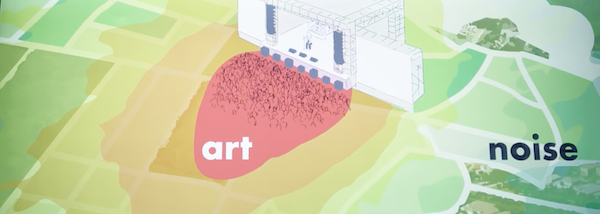
\includegraphics[width=1\textwidth]{change_later.png}
%	\caption{Normalized \gls{spl} in colour, red is high \gls{spl} where blue is low \gls{spl}}
%		\label{fig:Problem}
%\end{figure}
%
%%\autoref{fig:Problem} shows the total sound pressure level \gls{spl} in \gls{db} from \SI{20}{\hertz} to \SI{20}{\kilo\hertz} for the voluntary listeners and the non-voluntary listeners during a concert.
%\autoref{fig:Problem} shows a qualitative drawing of a near-ideal sound pressure distribution in the vicinity of a stage during a concert. The high-\gls{spl}areas are highlighted by red color, and is the area where the voluntary listeners condense. This area is define as the \textbf{participants' area} The non-voluntary listeners are located in the area around the participants' area, that we define as \textbf{the neighbourhood}. 
%
%While a \gls{spl} distribution as depicted in \autoref{fig:Problem} is easier to achieve the higher the frequency gets, towards low frequencies the \gls{spl}distribution might look more like depicted in autoref(fig:problem2).
%
%
%
%The directivity control of mid- and high frequency has a known solution which has been applied for many years. In general, horns are used, which are designed for a particular radiation pattern. Due to the long wave length in the low/mid- and low frequency range, the horns that are required to direct those wavelengths are not feasible for practical applications due to their size and weight. Therefore other, more space saving solutions have been developed and implemented in the last decade. It is possible to achieve a cardiod emission pattern by arranging subwoofers in a particular manner. Two or three subwoofers are pointed towards the participants' area and one subwoofer is pointed the opposite way \citep{KS28}. The signal for the subwoofer pointing away from the audience is processed to manipulate the phase.
%
%
%This project aims towards applying a principle that has been put into commercial use in the D\&B audiotechnik SL-series, where the low/mid frequency directivity is controlled by signal processing four speaker unit. Two units are arranged in the front of the line array module and the other two arranged on each of the sides of the line array module.



\section{Problem Statement}\label{sec:problem_statement}
Ideally, there would be a technique, that enables the user to take control of the directivity of sound emission from loudspeakers, making it possible to eliminate sound emission in a particular direction while keeping a linear frequency response in the direction, that sound is intended to be heard in. Noise pollution from outside music venues could be reduced to a fraction.\\
As of now, ambitions to addressing the problem begin to emerge in commercial products.
The goal of this project is developing an experimental low/mid frequency beamforming loudspeaker array. In order to comprehend the nature of the topic and investigate what order of magnitude the sound pressure attenuation can be achieved, the goal of this project is developing an experimental loud speaker array based on three loudspeakers placed in a triangular configuration.
In the course of doing so, the following aspects will be investigated:
\begin{itemize}
\item What are the directional characteristics of a single loudspeaker and in what frequency range can this be approximated as an omnidirectional sound source?
\item What model and/or simulation is suitable to predict the behaviour of the speaker array?
\item What placement of loudspeakers is suitable for beamforming in the intended frequency range?
\item Does the beamforming array improve the sound behaviour in a room?
\item How can \gls{sp}-parameters, that lead to beamforming with a chosen speaker configuration, be found and implemented?
\item After building the speaker array and measuring its directional characteristics, can the predictions given by the models be confirmed and what model gives the best estimates?
\item How does the implemented array compare to other low/mid frequency beamforming devices?
\end{itemize}

%The following questions are made with the intention of gathering the necessary knowledge, to be able to answer a later stated problem statement. The preliminary questions, which will be answered in the analysis, are:
%
%\begin{itemize}
%\item In which frequency area do the line source speaker behave omnidirectional?
%\item Which known technique is used to do the speaker cardioid?
%\item Can a simulation be made which support D\&B audiotechnik claim?
%\item Does beam forming of a line source speaker benefit in a room environment ?
%\end{itemize}



